\documentclass[12pt,a4paper]{report}

\usepackage[a4paper,margin=2.55cm]{geometry}
\usepackage{setspace}
\setstretch{1.58}
\usepackage{amsmath,amssymb}
\usepackage{booktabs,array,tabularx,longtable}
\usepackage{tikz}
\usetikzlibrary{arrows.meta,positioning,calc}
\usepackage{pgfplots}
\pgfplotsset{compat=1.18}
\usepackage{caption}
\usepackage{enumitem}
\usepackage[hidelinks]{hyperref}

\setlength{\parskip}{0.32em}
\setlength{\parindent}{1.15em}
\setlist[enumerate]{itemsep=0.22em,topsep=0.35em}
\setlist[itemize]{itemsep=0.22em,topsep=0.35em}
\captionsetup{font=small,skip=6pt}
\pgfplotsset{every axis/.append style={tick label style={font=\small},label style={font=\small}}}

\title{A Study on Improving Thresher Efficiency\\Using Deep Neural Networks}
\author{A computer-science thesis}
\date{}

\begin{document}
\maketitle
\thispagestyle{empty}

\begin{abstract}
\noindent
Threshing efficiency and mechanical stability are usually set by a fixed command or by a moisture card. Both ignore the axial load shape, and both are blind to an interaction between a heavy feed and a wet crop. This thesis treats the thresher as a plant and studies two computational problems on it. The first is to identify a discrete operating status from a short sensor window, after the axial stations have been placed by a design criterion rather than by habit. The second is to map the resulting features to four normalized setpoints---intensity, residence, cleaning, and feed admission---with a deep network trained to imitate a numerical optimizer.

The status model is a feedforward network on window statistics. On a held-out mixture of operating conditions it reaches \(89.8\%\) accuracy and a macro-F1 of \(0.846\), against \(82.6\%\) and \(0.734\) for a linear softmax on the same features. The gain is concentrated on the spatial and the rare labels: front-loaded recall rises from \(0.56\) to \(0.79\), and under-filled recall from \(0.27\) to \(0.61\). A \(D\)-optimal design for a quadratic load shape puts stations at the inlet, at two central bands, and at the discharge. Accuracy saturates once the two ends are instrumented, which is what a contrast feature needs; the four-station design is kept because the control features also use the curvature of the load.

The control network is trained by squared error against the optimizer, on features drawn under a fixed command, under the moisture card, and under random commands. On a weighted seasonal mix of wheat, rice, and soybean it lowers grain loss from \(2.85\%\) at the fixed setting and \(2.50\%\) on the moisture card to \(1.80\%\), against \(1.78\%\) for the optimizer itself. Specific shaft energy rises from \(1.41\) to \(1.63\,\mathrm{kWh\,t^{-1}}\). A stability index whose design floor is \(0.70\) rises from \(0.686\) to \(0.701\). Impurity rises from \(1.17\%\) to \(1.50\%\) and a breakage index from \(1.04\%\) to \(1.49\%\). Those two rises are the prices inside the optimizer's objective, not side effects discovered after the fact. The numbers are a numerical experiment on a reduced-order plant. They are not a field trial.
\end{abstract}

\tableofcontents
\newpage

\chapter*{Nomenclature}
\addcontentsline{toc}{chapter}{Nomenclature}
\markboth{Nomenclature}{Nomenclature}

Symbols used in more than one place are collected here. A symbol that belongs to a single derivation is defined where it appears.

\begin{longtable}{@{}p{0.16\textwidth}p{0.76\textwidth}@{}}
\toprule
Symbol & Meaning \\
\midrule
\endhead
\(q\) & Fresh biomass feed offered to the machine, kilograms per second. \\
\(m\) & Grain moisture, wet basis, as a fraction. \\
\(u_I,u_R,u_C,u_F\) & Normalized commands: threshing intensity, residence, cleaning, and feed admission, each in \([0,1]\). \\
\(\mathbf{u}\) & The command vector \((u_I,u_R,u_C,u_F)\). \\
\(\mathbf{u}^\star\) & Command returned by the numerical optimizer for a known disturbance. \\
\(q_e\) & Biomass actually admitted to the rotor after the feed trim. \\
\(\eta\) & Grain-recovery efficiency: recovered grain divided by grain offered. \\
\(L\) & Grain-loss fraction of the admitted grain. The sum of unthreshed, free-grain, and sieve terms. \\
\(\iota\) & Impurity fraction in the cleaned stream. \\
\(b\) & Breakage index, a monotone function of residence, intensity, and moisture. \\
\(e\) & Specific shaft energy, kilowatt-hours per tonne of admitted grain. \\
\(F_i\) & Load at axial station \(i\), newtons. Stations are numbered \(1\) to \(8\) from inlet to discharge. \\
\(\mathrm{CV}\) & Coefficient of variation of the station loads. \\
\(S\) & Mechanical-stability index in \([0,1]\). Higher is calmer. The design floor is \(0.70\). \\
\(\mathbf{x}\) & Feature vector built from one sensor window. \\
\(p\) & The set of axial stations that are instrumented. \\
\(K\) & Number of instrumented axial stations. \\
\(C\) & Discrete operating status. \\
\(J\) & Scalar objective maximized by the teacher optimizer. \\
\bottomrule
\end{longtable}

\chapter{Background and Problem Statement}
\label{ch:back}

The machine in this thesis is a thresher. The contribution is not a new machine. It is a pair of computations that a fixed setting and a moisture card do not perform: a placement of sensors and a feature model that identify the operating status, and a deep network that turns those features into commands which raise grain recovery while a stability floor, an energy price, an impurity price, and a breakage price remain in force. This chapter says what the plant is, what the published learning systems already do with machines of this kind, and which two problems the later chapters are required to answer.

\section{Structure, Operating Principles, and Types of Threshers}
\label{sec:plant}

\subsection{What the computer is allowed to mean by the machine}

A thresher frees grain from ears or pods and delivers the grain without the straw. Operators learn a setting on a uniform crop and leave it there while the feed and the moisture change. A moisture card is the same habit written down: wetter grain is given a harder or a longer pass, and the card does not read the load. The computer-science object is the map from a window of measurements to the next command. The metal exists in this thesis only so that the map has inputs, outputs, and a cost.

The topology used from here on has four blocks. A feeder admits biomass. A threshing unit applies impact and rubbing against a concave, and grain that is free can leave through that concave. A cleaner, made of air and oscillating sieves, then accepts grain and rejects chaff. Material that the cleaner does not decide may be offered to the inlet again. Straw leaves at the rear. Figure~\ref{fig:flow} is that topology drawn as a plant, with the quantities the later chapters actually name.

\begin{figure}[ht]
\centering
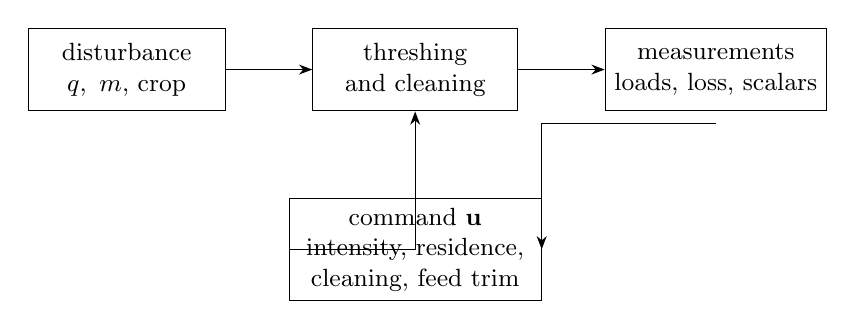
\begin{tikzpicture}[>=Stealth,node distance=8mm,font=\small]
  \node[draw,align=center,minimum width=2.5cm,minimum height=1.05cm] (d) {disturbance\\ \(q,\ m,\) crop};
  \node[draw,align=center,right=11mm of d,minimum width=2.6cm,minimum height=1.05cm] (p) {threshing\\and cleaning};
  \node[draw,align=center,right=11mm of p,minimum width=2.7cm,minimum height=1.05cm] (y) {measurements\\loads, loss, scalars};
  \node[draw,align=center,below=11mm of p,minimum width=3.2cm,minimum height=1.05cm] (c) {command \(\mathbf{u}\)\\intensity, residence,\\cleaning, feed trim};
  \draw[->] (d) -- (p);
  \draw[->] (p) -- (y);
  \draw[->] (y.south) ++(0,-0.15) -| (c.east);
  \draw[->] (c.west) -| (p.south);
\end{tikzpicture}
\caption{The thresher as the plant used in this thesis. The learning method sees a disturbance, a measurement window, and a four-dimensional command. It does not redesign the mechanism that realizes the command.}
\label{fig:flow}
\end{figure}

\subsection{Operating principle, stated as quantities}

Three failures define a bad pass, and they are different failures. Grain that is still attached when the straw leaves is an unthreshed loss. Free grain that is still in the straw is a separation loss. Grain that the cleaner throws away is a sieve loss. Chaff that stays in the sample is impurity, which is not a loss of grain and must not be added to one. A faster or a longer pass can cut the first two losses and can crack kernels. A more open cleaner can cut the third loss and can raise impurity. Power rises with intensity and with residence. None of these signs is controversial; they are the reason a single knob is not a controller \cite{fu2018,miu2008a,harrison1991}.

Mechanical stability, as the word is used here, is not a stress analysis of a shaft. It is an index of the running machine. The axial load should not pile up at the inlet while the discharge runs light. The peak load should stay clear of a blockage level. Vibration should stay in proportion to the intensity that was asked for. Chapter~\ref{ch:method} writes the index \(S\in[0,1]\) from those three signals and puts a floor under it. A command that buys recovery by crossing the floor is a failed command even if the loss number looks better.

The feed and the moisture do not act as separate additives. A heavy feed on a dry crop and a heavy feed on a wet crop are different plants: the wet, heavy case packs the inlet and raises unthreshed loss together, which is a product, not a sum. A card that is linear in moisture cannot represent a product. That algebraic fact is the reason a linear command map is kept in the study as an ablation rather than assumed to be enough.

\subsection{Types, and why the axial plant is the one that is simulated}

Published descriptions group threshers by the path of the crop \cite{srivastava2006,kepner1978,fu2018}.

A tangential machine presents the crop to a drum for a fraction of one revolution. The concave is short. Separation after the drum is done by a straw walker or by a rotary separator. There is little axial shape to measure on the drum itself, and a single load on the concave is a fair summary of that station. The control problem then collapses toward a choice of drum speed and a single gap.

An axial machine keeps the crop in a cylindrical cage for many revolutions. Helical guides set how fast the mat walks from inlet to discharge. The load then has a shape. The inlet carries the full straw and the still-attached grain. The discharge carries straw and whatever free grain has not yet left. A uniform transport speed makes a front-heavy shape, because grain is leaving along the axis while the straw is not. One load cell on the whole concave sees the sum and misses the shape. A row of stations sees the shape. That row is a placement problem: which stations, and how many, are worth the channels.

A hold-on or stationary thresher changes the feeder and not the maps. The inlet may be a belt or a person rather than a header. Unthreshed loss, separation loss, sieve loss, impurity, and power still move with moisture and with how hard and how long the crop is worked. The sensor question is unchanged whenever the threshing unit is axial.

The numerical plant in Chapters~\ref{ch:method} and~\ref{ch:est} is axial, with eight possible load stations along the cage. The tangential machine is the comparison that explains the placement problem. It is not simulated. The stationary feeder is the reason feed admission is a command at all: the computer may trim the inlet for a short time without claiming to drive a vehicle.

\subsection{The interface the rest of the thesis is allowed to use}

The disturbance is the crop, the offered biomass feed \(q\), and the moisture \(m\). Three crops appear: wheat, rice, and soybean. They differ by grain fraction, by a difficulty multiplier on the loss and breakage maps, and by a multiplier on the load. They do not differ by a change of network architecture.

The command is four numbers in the unit interval. Intensity \(u_I\) stands for how hard the threshing unit hits. Residence \(u_R\) stands for how long the mat is kept over the concave. Cleaning \(u_C\) stands for how aggressively the air-and-sieve stage sorts. Feed admission \(u_F\) trims the inlet over a limited range; it is not a license to shut the machine and call the idle state efficient. The mechanism that turns these four numbers into a rotor speed, a transport setting, a sieve, and a feeder speed is outside the learning method. The simulator in Chapter~\ref{ch:method} is the only place they have a numerical effect.

The measurement window contains the instrumented station loads, a shaft torque, a housing vibration, a sieve-loss proxy, a return flow, shaft power, moisture, and feed. Torque and power see the level of the load. They do not see which station is hot. Vibration is taken at the housing and is modeled as a function of intensity, moisture, and throughput, not of the axial peak. The peak's location is left to the stations. That split is deliberate. If a scalar sensor already contained the shape, a paper about placement would be arguing with its own sensor model.

Grain-recovery efficiency is recovered grain divided by grain offered. Cutting the feed lowers it, so a policy cannot improve the headline number by refusing crop. Grain loss \(L\) is the fraction of admitted grain that is unthreshed, free at the rear, or thrown by the cleaner. When the feed trim is fully open the two statements differ only by rounding. Specific energy \(e\) is shaft energy per tonne of admitted grain. Chapter~\ref{ch:est} also reports the shaft power that this specific energy implies, so the two cannot drift apart unnoticed.

\section{Artificial Intelligence Applied to Threshers}
\label{sec:review}

\subsection{What the surveys already separate}

Two surveys of learning in agriculture, and one survey of combine control, are enough to locate the gap. Kamilaris and Prenafeta-Bold\'u group deep models in the field by the task the network is asked to perform, and the mass of the work is perception: weeds, fruit, disease, and land cover, with convolutional networks on images \cite{kamilaris2018}. Liakos and co-authors make the same cut from the other direction. Machine learning in agriculture is mostly yield, disease, and species decisions, and the machinery papers are a thin slice beside them \cite{liakos2018}. Chen, Qian, Jin, and Yang review control algorithms on grain combines and find the opposite emphasis: rotor speed, sieve opening, fan speed, and ground speed, closed one loop at a time, with learning used where a model of the cleaner or the header is inconvenient \cite{chen2025}. Perception papers and actuator papers cite each other and solve different problems.

A third survey, on vision for grain crops, makes the perception side concrete. Counting kernels, locating unthreshed heads, and scoring impurity from an image are detection problems, and the published systems treat the detector's output as the product \cite{patricio2018}. A detector can name a loss. It does not by itself choose a command vector under a stability floor.

\subsection{Loss sensing and single-loop control}

Impact plates under a sieve made grain loss a real-time count rather than a bag weighed at the end of a row. Liang, Li, Xu, and Zhao built that sensor for rice and studied where along the sieve a plate has to sit if the count is to stand for the shoe \cite{liang2016}. Zhao, Li, Chen, and Xu had already closed a monitoring loop of the same family \cite{zhao2011}. These papers are about observability of one term. They are not about the axial shape, and they are not about a joint command.

The cleaning controller that still structures the actuator literature is the fuzzy system of Craessaerts, De~Baerdemaeker, Missotten, and Saeys \cite{craessaerts2010a}. It trades sieve loss, return volume, and impurity, and it moves a fan and a sieve opening. Return volume is a penalty in the cost. It is not a delayed state. Shoe frequency, stroke, and a gate are outside the command. The identification underneath the controller was done with the rotor held in one condition, so the axial load never enters the features.

Model-predictive cruise control on the combine, as in the Leuven line, moves ground speed from a process model and a horizon \cite{coen2008b,rawlings2017}. It is the right computation when the command is a speed and the constraint is a capacity. It is a different command from the four setpoints in this thesis, and it assumes a model the designer already trusts at the horizon. The optimizer in Chapter~\ref{ch:method} is in that computational family: a numerical minimization of a scalar cost subject to bounds \cite{nocedal2006}. It is used as a teacher, offline, with the disturbance known. It is not proposed as the program that has to run from a noisy window every control period.

\subsection{What is not in those papers}

The published pieces can be lined up without caricature.

\begin{itemize}
\item A vision or impact model estimates a loss or an impurity. The estimate is the output.
\item A fuzzy or predictive loop moves one or two actuators. The axial load shape is not a feature, and a stability floor on that shape is not a constraint.
\item A threshing balance of the Miu--Kutzbach kind predicts loss along a machine once the rates are known \cite{miu2008a}. It is a plant model. It does not place sensors, and it does not approximate its own optimizer with a network.
\end{itemize}

Two computational objects are missing from that list. The first is a placement. Eight possible stations and a budget \(K\) are a design of experiments on a shape model \cite{atkinson2007}, followed by a check of whether the status labels that the shape induces are actually recovered by a classifier. The second is a function from the resulting features to the teacher's command. The teacher can afford a numerical solve with the true disturbance in hand. The onboard program cannot. A feedforward network is a standard approximant of a continuous map on a compact set \cite{cybenko1989,hornik1991,goodfellow2016}. Whether this particular map needs the depth, or whether a linear map on the same features already matches it, is an empirical question the study is required to answer rather than to assume. The status boundary is a different question. Front-loaded, blockage-risk, and high-loss share some of the same sensors and are separated by thresholds on different quantities. A linear softmax and a small ReLU network do not have to tie on that boundary \cite{bishop2006,hastie2009}.

Recurrent networks are the right tool when the raw series is the input and the relevant time is long \cite{lecun2015}. Here the window is short and is reduced to statistics before the network sees it. The architecture that matches that choice is feedforward. Chapter~\ref{ch:method} does not train a recurrent net and then claim a comparison it did not run.

\section{Problems Addressed by This Thesis}
\label{sec:problems}

\subsection{Problem 1: status from a designed placement}

Let \(C\) be a label in
\[
\{\text{stable},\ \text{front-loaded},\ \text{under-filled},\ \text{blockage-risk},\ \text{high-loss}\},
\]
assigned from the full load shape, the loss, and the mean load by the priority rule in Chapter~\ref{ch:method}. The rule uses the true stations. The classifier does not. It sees a window from a subset \(p\) of the eight stations, together with the scalar channels that are always present.

\textbf{Problem 1.} Choose a placement \(p\) with \(|p|=K\), a feature map \(\mathbf{x}\), and a classifier \(\hat C(\mathbf{x})\), so that \(\hat C\) recovers \(C\) on conditions that were not used to choose \(p\). Report accuracy and macro-F1 against a linear softmax on the same features, and report the same figures for a placement that simply takes the first \(K\) stations from the inlet. A design that raises accuracy by memorizing the training windows is not a solution. The test mixture is drawn again, with new noise.

The label set is part of the problem. Accuracy alone is a weak score because a stable machine is the common case. Macro-F1 gives the rare labels a vote. Under-filled is the thinnest class in the test mixture, and its recall is reported with that fact attached.

\subsection{Problem 2: commands that raise recovery under a priced stability floor}

Let \(\mathbf{u}^\star(q,m,\text{crop})\) be a maximizer of the objective \(J\) defined in Chapter~\ref{ch:method}. The maximizer may use the true disturbance. The network may not. It receives \(\mathbf{x}\) built from a noisy window that was generated under some other command, and it emits \(\hat{\mathbf{u}}(\mathbf{x})\).

\textbf{Problem 2.} Train \(\hat{\mathbf{u}}\) so that the closed-loop plant, under \(\hat{\mathbf{u}}\), improves grain loss relative to a fixed command and relative to a moisture card, keeps the seasonal mean of \(S\) at the floor \(0.70\) rather than under it, and stays close to the teacher's loss, energy, impurity, and breakage. A solution that cuts loss by refusing feed, or by idling the rotor, fails the definition of \(\eta\) and fails \(J\). A solution that matches the teacher on average and misses the wet, heavy row by a wide margin must say so in the point table. The linear map on the same features is the ablation that decides whether depth is doing work on this command or only on the status label.

\subsection{Requirements the later chapters are checked against}

\begin{enumerate}[label=R\arabic*.]
\item The placement is chosen by a stated criterion on a shape model, and the installed set is written down as station numbers.
\item The status model and the command model are trained on one sample and scored on another. The seasonal points used in Chapter~\ref{ch:est} are not the training set.
\item The command model does not receive \(C\) as an input. Status and command are separate networks that share a feature definition. A hidden leak of the true label into \(\hat{\mathbf{u}}\) would make Problem~2 a different problem.
\item Feed admission may move only inside the trim encoded by the plant. Recovery is computed on grain offered, so a closed trim is a loss of recovery.
\item Energy, impurity, and breakage are reported beside loss. A table that shows only loss is not an answer to Problem~2.
\item The onboard program specified in Chapter~\ref{ch:est} is a fixed cyclic schedule: build the window, standardize, evaluate the two networks, and rate-limit the write. It does not call the teacher.
\item Claims are limited to the reduced-order plant. A field percentage is not among the results.
\end{enumerate}

\subsection{Assumptions that bound the claims}

\begin{enumerate}[label=A\arabic*.]
\item The plant maps in Chapter~\ref{ch:method} are smooth, static, and first-order in the losses. A rate that saturated harder at high load would move the wet-rice numbers. It would not remove the product between feed and moisture that the linear card cannot see.
\item Station noise, torque noise, and the loss-proxy noise are independent and zero-mean at the variances written with the feature map. A shared electrical fault would break the median-free design used here; the program's response to a missing station is specified separately and is not claimed to cover a stuck-at bias that looks like a real load.
\item The teacher is a local bound-constrained solve started from a coarse grid \cite{nocedal2006}. A better global search could move a point. The network is trained to imitate the teacher that was actually run.
\item The moisture card is a competent linear policy, not a straw man. It is allowed to beat the fixed setting on wet crops. It is not given the feed or the load shape.
\item No grain price and no fuel price enter \(J\). The weights are design choices, published so the tables can be read against the cost that produced them. Changing the breakage weight would move residence. The comparison among fixed, card, linear map, network, and teacher is at one published weight vector.
\item The network is a static map of one window. It has no internal state beyond the rate limit applied at the write. A slower drift of moisture than the window is handled because moisture is itself a feature, not because the network remembers the morning.
\end{enumerate}

\subsection{What the later chapters owe this statement}

Chapter~\ref{ch:method} writes the plant, the features, the \(D\)-criterion, the two networks, and the offline scores: classification against the linear softmax, and command error against the teacher. Chapter~\ref{ch:est} writes the cyclic program that would run those networks, and the closed-loop numbers on the seasonal mix and on one feed transient. A result that appears only as a training loss is not yet a result of Problem~2. Problem~2 is about the plant after the command is applied.

\chapter{Application of Deep Neural Networks to Enhance Threshing Efficiency}
\label{ch:method}

The problems in Chapter~\ref{ch:back} ask for a placement, a feature map, a status model, and a command model. This chapter defines them and scores them offline. The plant comes first, because every label and every teacher command is a function of it. The plant is a reduced-order simulator. It is not a derivation from a new experiment, and it is not a sizing of hardware. Its only duty is to land a fixed command in the loss and specific-energy band already published for axial machines, and to contain the feed--moisture product that a linear card cannot represent \cite{miu2008a,harrison1991}.

\section{Positioning Sensors to Identify Operating Status}
\label{sec:place}

\subsection{Indicators, and the ones that were refused}

Operating status is a label of the running machine, not a name for the crop. Five labels are used, and they are assigned from the true plant output in this priority, so the first match wins:

\begin{enumerate}
\item blockage-risk, if the peak station load is at least \(0.84\times 1680\,\mathrm{N}\);
\item high-loss, if grain loss is at least \(2.8\%\);
\item front-loaded, if the inlet station exceeds the discharge station by at least \(0.38\) of the mean load and the peak is at least \(760\,\mathrm{N}\);
\item under-filled, if the mean station load is at most \(430\,\mathrm{N}\);
\item stable, otherwise.
\end{enumerate}

The priority is the model of ``what an operator would say first.'' A machine that is both front-loaded and past the blockage line is blockage-risk. A machine that is merely light is under-filled only if no sharper failure is present.

The indicators that can see these labels are not a catalog of every transducer on a combine. They are the smallest set whose absences are informative.

\begin{itemize}
\item Axial station loads see the level, the peak, and the contrast. Without at least two stations that are far apart, front-loaded is not a measurement.
\item Shaft torque and shaft power see the level a second time. They do not see which station produced it. They stay in the feature vector as scalars that are always installed.
\item Housing vibration sees intensity, moisture, and throughput. In the simulator it does not depend on the peak station. Putting the peak into the vibration channel would have made the placement study circular.
\item A sieve-loss proxy sees the cleaner term that high-loss partly reflects. It does not see the axial shape.
\item Return flow is kept because it moves with sieve loss and is cheap. It is not a separate label.
\item Moisture and offered feed are measured directly. They are disturbances, and they are also legitimate features, because the onboard program is allowed to read the sensors the machine already has for them.
\end{itemize}

A camera is not in the set. Problem~1 is about whether a short physical window, after a placement decision, is enough for the five labels. Adding an image channel would answer a different question, the one the perception surveys have already framed \cite{kamilaris2018,patricio2018}.

\subsection{The load shape the placement is designed for}

Index the eight stations by \(\xi_i=i/7\) for \(i=0,\ldots,7\), so the inlet is \(0\) and the discharge is \(1\). The design model treats the load along the axis as a quadratic plus noise,
\begin{equation}
F(\xi) = \theta_0 + \theta_1 \xi + \theta_2 \xi^2 + \varepsilon,
\qquad
\phi(\xi) = (1,\ \xi,\ \xi^2)^\top .
\label{eq:shape}
\end{equation}
For a placement \(p\), the Fisher information of an independent, equal-variance sample is
\begin{equation}
M(p) = \sum_{i\in p} \phi(\xi_i)\,\phi(\xi_i)^\top .
\label{eq:fisher}
\end{equation}
The \(D\)-optimal placement of size \(K\) maximizes \(\det M(p)\) \cite{atkinson2007}. With fewer than three stations the quadratic is singular, so the two-station design is computed on the line \(\phi(\xi)=(1,\xi)^\top\) instead. The criterion then puts the two sensors at the ends of the interval, which is the classical answer for a slope, and it is also the pair a contrast feature needs.

The designs that win are:

\begin{table}[ht]
\centering
\caption{\(D\)-optimal station sets. Station \(1\) is the inlet and station \(8\) is the discharge. The determinant column is \(\det(M)^{1/3}\) for the quadratic model. The two-station row is a different model and is not numerically comparable to the others.}
\label{tab:dopt}
\begin{tabular}{@{}cll@{}}
\toprule
\(K\) & Stations & Quadratic \(\det(M)^{1/3}\) \\
\midrule
2 & 1, 8 & (line model) \\
3 & 1, 4, 8 & 0.391 \\
4 & 1, 4, 5, 8 & 0.497 \\
5 & 1, 2, 4, 5, 8 & 0.568 \\
6 & 1, 2, 4, 5, 7, 8 & 0.651 \\
8 & all & 0.783 \\
\bottomrule
\end{tabular}
\end{table}

The pattern is the one the polynomial asks for. The ends identify level and slope. A station near the middle identifies curvature. Extra stations cluster beside those three rather than filling the cage uniformly. The installed design is the four-station set \(\{1,4,5,8\}\). It is the smallest quadratic design that has both a middle pair and the two ends. Section~\ref{sec:simoff} checks whether a classifier wants a very different set. It does not, once the score is accuracy on these five labels: two well-separated stations already carry the contrast, and further stations do not create a sixth label.

\begin{figure}[ht]
\centering
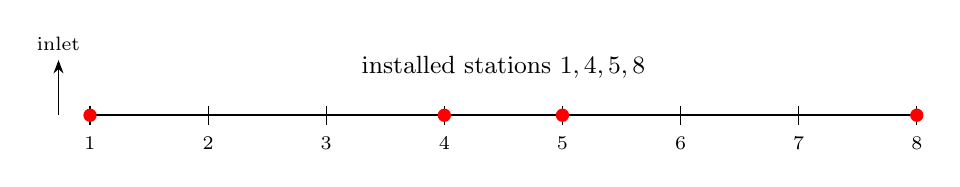
\begin{tikzpicture}[>=Stealth]
  \draw[thick] (0,0) -- (10.5,0);
  \foreach \i/\x in {1/0, 2/1.5, 3/3.0, 4/4.5, 5/6.0, 6/7.5, 7/9.0, 8/10.5} {
    \draw (\x,0.12) -- (\x,-0.12);
    \node[below] at (\x,-0.15) {\scriptsize \i};
  }
  \foreach \x in {0, 4.5, 6.0, 10.5} {
    \fill[red] (\x,0) circle (2.4pt);
  }
  \node[above] at (5.25,0.35) {\small installed stations \(1,4,5,8\)};
  \draw[->] (-0.4,0) -- (-0.4,0.7) node[above,font=\scriptsize]{inlet};
\end{tikzpicture}
\caption{The eight candidate stations and the four that the \(D\)-criterion installs. The inlet is station \(1\).}
\label{fig:stations}
\end{figure}

\subsection{The feature map}

A window is eight samples. At the \(20\,\mathrm{Hz}\) rate used by the program in Chapter~\ref{ch:est}, the window is \(0.4\,\mathrm{s}\). For each installed station the features are the window mean and the window standard deviation. From the vector of means the map adds the coefficient of variation, the contrast between the first and the last installed station divided by the mean, and the maximum mean. Torque, vibration, the loss proxy, return flow, and power each contribute a mean and a standard deviation. Moisture and feed contribute one noisy reading each. Loads are divided by \(1000\), load standard deviations by \(100\), the loss proxy is multiplied by \(100\), power's mean is divided by \(10\), and feed is divided by \(10\), so that a standardized network does not have to spend its first epochs on units. With four stations the raw feature dimension is \(23\).

The noise used when the windows are drawn is part of the method, not a hidden robustness trick. Station loads are perturbed by independent Gaussian noise of standard deviation \(22\,\mathrm{N}\). Torque, vibration, loss proxy, return, and power use standard deviations \(0.015\), \(0.03\), \(0.0015\), \(0.012\), and \(0.15\) in the units of those channels. Moisture noise is \(0.004\) and the scaled-feed noise is \(0.012\). A stuck channel is not this noise. It is the fault case in Chapter~\ref{ch:est}.

Standardization is affine and is fit on the training windows only:
\begin{equation}
\tilde{\mathbf{x}} = (\mathbf{x}-\boldsymbol{\mu}_{\mathrm{tr}})\oslash \boldsymbol{\sigma}_{\mathrm{tr}},
\label{eq:std}
\end{equation}
with any coordinate whose training standard deviation is below \(10^{-6}\) left unscaled. The same \(\boldsymbol{\mu}_{\mathrm{tr}}\) and \(\boldsymbol{\sigma}_{\mathrm{tr}}\) are applied to validation, test, and the closed-loop program. Refitting them on the test mixture would leak the evaluation into the preprocessor.

\subsection{The status network}

The status model is a feedforward net with sizes \(23\)--\(48\)--\(32\)--\(5\). Hidden layers are ReLU. The output is a softmax. Initialization is Gaussian with variance \(2/n_{\mathrm{in}}\) on each layer, the scale that keeps ReLU layers from starting saturated \cite{he2015}. Training minimizes the multinomial cross-entropy with Adam at learning rate \(8\times 10^{-4}\), batches of \(64\), for \(100\) epochs \cite{kingma2015,rumelhart1986}. The epoch with the best validation accuracy is the one that is kept. On the run reported here that epoch is \(99\). The network has \(2885\) parameters.

The linear baseline is a softmax with the same standardized input, no hidden layer, trained by minibatch gradient descent with \(\ell_2\) weight \(10^{-3}\). It is the correct baseline. A gain of the deep model over a different feature set would not answer Problem~1.

Labels for training are computed from the noise-free plant at the command that produced the window. The command is not always the teacher's command. Each disturbance is observed three times: under the fixed setting, under the moisture card, and under a command drawn uniformly from \([0.15,0.95]^4\). A classifier trained only at the fixed setting would not be entitled to a score on the other two, and the program in Chapter~\ref{ch:est} has to recognize status while it is in the middle of changing the command.

\section{A Deep Network for Efficiency and Mechanical Stability}
\label{sec:net}

\subsection{The simulator the teacher optimizes}

The command \(\mathbf{u}=(u_I,u_R,u_C,u_F)\) and the disturbance \((q,m)\) enter a static map. Admitted biomass is the trim
\begin{equation}
q_e = q\,(0.82 + 0.18\,u_F),
\label{eq:qe}
\end{equation}
so a fully closed trim still passes \(82\%\) of the offer. Define \(q_n=\mathrm{clip}(q_e/6,\ 0.35,\ 1.8)\) and the packing interaction
\begin{equation}
\pi = \frac{1}{0.08}\,\max(q_n-0.75,\ 0)\,\max(m-0.16,\ 0).
\label{eq:pack}
\end{equation}
Packing is zero when the feed is light or the crop is dry. It is large only when both are high, and several loss and load terms below are multiplied by a factor that falls as residence rises. A model that is linear in \(q\) and linear in \(m\) does not contain \(\pi\).

Unthreshed loss, free-grain loss, and sieve loss, as fractions of admitted grain, are
\begin{align}
L_u &= 0.058\, d_c\, e^{-3.40 u_I}\, e^{-0.85 u_R}\, e^{6.4(m-0.15)}\, q_n^{0.58}\,
        e^{0.70\pi \max(0.80-u_R,\ 0)}, \label{eq:lu}\\
L_g &= 0.026\, d_c\, e^{-2.05 u_R}\, e^{-0.30 u_I}\, e^{4.0(m-0.15)}\, q_n^{0.46}\,
        e^{0.50\pi \max(0.78-u_R,\ 0)}, \label{eq:lg}\\
L_s &= 0.0125\, e^{-2.05(u_C-0.18)}\, e^{2.8\max(m-0.18,\ 0)}\, q_n^{0.58}\,
        \big(1.08+0.28(1-u_I)\big). \label{eq:ls}
\end{align}
Impurity and breakage are
\begin{align}
\iota &= 0.0108\, e^{1.70(u_C-0.40)}\, e^{-0.45(u_I-0.50)}\, (0.80+1.05\,m), \label{eq:iota}\\
b &= 0.0034\, d_c\, e^{1.90 u_R}\, e^{0.38 u_I}\, e^{2.7\max(m-0.18,\ 0)}. \label{eq:b}
\end{align}
Grain loss is \(L=L_u+L_g+L_s\). Recovery charges the trim,
\begin{equation}
\eta = (q_e/q)\,(1-L).
\label{eq:eta}
\end{equation}
Specific energy, in \(\mathrm{kWh\,t^{-1}}\) of admitted grain, is
\begin{equation}
e = (0.58 + 0.72\,u_I + 0.62\,u_R)\,
    \big(1+2.15(m-0.14)\big)\,
    (0.90+0.16\,d_c)\,
    (0.94+0.08\,q_n).
\label{eq:energy}
\end{equation}
Shaft power in kilowatts is \(P = 3.6\, e\, q_e\, \phi\), with \(\phi\) the grain fraction. The factor \(3.6\) is the unit change from kilograms per second and kilowatt-hours per tonne into kilowatts. Crop coefficients are \(\phi\), difficulty \(d_c\), and a load scale \(s_F\): wheat \((0.46,\ 1.00,\ 1.00)\), rice \((0.41,\ 1.28,\ 1.12)\), soybean \((0.55,\ 0.86,\ 0.92)\).

Station loads use the same packing term. With inlet and discharge shape factors
\begin{equation}
s_{\mathrm{in}} = 1.55 - 0.58\,u_R + 0.42\,\pi\max(1-u_R,\ 0),
\qquad
s_{\mathrm{out}} = 0.70 + 0.34\,u_R,
\label{eq:shapeends}
\end{equation}
the load at \(\xi\) is proportional to
\(s_{\mathrm{in}}+(s_{\mathrm{out}}-s_{\mathrm{in}})\xi\), to a small curvature that packing adds, to \(q_e\), to moisture, to a weak intensity factor \((0.86+0.28\,u_I)\), and to \(s_F\). The constant of proportionality is \(720\,\mathrm{N}\) at the reference point \(q_e=6\), \(m=0.14\), \(u_I=0\), and a flat unit shape. Residence is what moves the shape. Intensity is what moves unthreshed loss. The two commands are not substitutes, which is the reason both exist.

Housing vibration is
\begin{equation}
v = \big(0.20 + 0.88\,u_I^{1.30}\big)\,
    \big(1+3.4\max(m-0.20,\ 0)\big)\,
    (0.85+0.20\,q_n).
\label{eq:vib}
\end{equation}
The stability index clips each of three normalized terms and then clips the sum:
\begin{equation}
\begin{aligned}
S = \mathrm{clip}\big(&1 - 0.40\,\mathrm{clip}(\mathrm{CV}/0.42,\ 0,\ 1.35)
 - 0.32\,\mathrm{clip}(v/1.55,\ 0,\ 1.35) \\
&- 0.28\,\mathrm{clip}\big((F_{\max}/1680-0.48)/0.62,\ 0,\ 1.35\big),\ 0,\ 1\big).
\end{aligned}
\label{eq:stab}
\end{equation}
\(\mathrm{CV}\) is the coefficient of variation of the eight station loads, whether or not all eight are instrumented. The index is a property of the plant. The features see only the installed stations.

\subsection{The objective the teacher maximizes}

The teacher solves, for known \((q,m,\text{crop})\),
\begin{equation}
\begin{aligned}
\max_{\mathbf{u}\in[0,1]^4}\ 
J = \eta &- 0.012\,e - 0.48\,\iota - 1.15\,b - 0.025\,\mathrm{CV} \\
&- 0.26\,\max(0,\ 0.70-S)
- 0.40\,\max\!\big(0,\ F_{\max}/1680-0.82\big)^2 .
\end{aligned}
\label{eq:J}
\end{equation}
Recovery is the thing to raise. Energy, impurity, and breakage are prices per unit, so a longer, harder, cleaner pass has to pay. The coefficient of variation has a small linear price. The stability term is a hinge at \(0.70\): once the index is above the floor it contributes nothing further, and the teacher is free to spend margin that a timid setting had left unused. The blockage term is a squared hinge at \(82\%\) of \(1680\,\mathrm{N}\). The weights are not fitted to a preference study. They are the cost for which every table in Chapter~\ref{ch:est} was generated. Assumption A5 of Chapter~\ref{ch:back} is this sentence.

The solve is a four-level grid on \([0.15,0.90]^4\), then a bound-constrained quasi-Newton polish from the best grid point \cite{nocedal2006}. The grid makes the start cheap and keeps a bad local basin from being the only basin that is tried. The teacher is still local. Problem~2 imitates this teacher, not an unseen global solver.

The fixed command, used as one baseline, is \((0.50,\ 0.44,\ 0.46,\ 1)\). The moisture card, used as the other, is
\begin{equation}
\begin{aligned}
u_I &= \mathrm{clip}\big(0.50+1.25(m-0.15),\ 0.38,\ 0.82\big),\\
u_R &= \mathrm{clip}\big(0.46+1.15(m-0.15),\ 0.32,\ 0.80\big),\\
u_C &= \mathrm{clip}\big(0.47+0.85(m-0.16),\ 0.36,\ 0.70\big),\\
u_F &= 1,
\end{aligned}
\label{eq:card}
\end{equation}
and it does not read \(q\) or any load. On a wet crop it raises intensity, residence, and cleaning together. On a dry, heavy crop it does the wrong thing for the feed, because the moisture is low and the feed is invisible. That row is kept in the seasonal mix for that reason.

\subsection{The command network}

The command model is a second feedforward net, sizes \(23\)--\(64\)--\(64\)--\(32\)--\(4\), ReLU hidden units, linear output, clipped to \([0,1]\) when it is applied. It has \(7908\) parameters and \(7744\) multiply-adds. The same He-style initialization and the same Adam settings are used, with learning rate \(10^{-3}\) for \(140\) epochs \cite{he2015,kingma2015}. The kept epoch is the one with the lowest validation mean squared error, epoch \(122\) in the reported run, where that error is \(1.03\times 10^{-3}\).

The target is \(\mathbf{u}^\star\). The input is not the feature window at \(\mathbf{u}^\star\). Each training disturbance contributes three windows, generated under the moisture card, under a random command, and under the fixed command, all labeled with the same \(\mathbf{u}^\star\). A network trained only at the teacher's own operating point would be asked, at deployment, to act from the card's operating point, which is a different distribution of features. One mixture of the three conditions is the whole of the correction used here. It is in the spirit of dataset aggregation and it is not an iterated online reduction \cite{ross2011}. Calling it a no-regret imitation loop would overstate a single static sample.

The linear ablation is least squares from the standardized features, plus a bias, onto \(\mathbf{u}^\star\), with the prediction clipped to \([0,1]\). Same inputs, same targets, no hidden layer. If this map matches the network on the plant, depth is not what moves the grain, and the thesis has to say that.

The loss that is trained is squared error on the four commands. It is not \(J\), and it is not a reinforcement signal. The teacher has already folded \(J\) into \(\mathbf{u}^\star\). Training on \(J\) directly would be a different algorithm and would need the plant inside the training loop. Imitation is the algorithm that matches requirement R6: the onboard program evaluates a function and does not call the teacher.

\subsection{What the command network is not}

It does not take the status label as an input. A correct label would be a strong feature and would glue Problem~1 to Problem~2 so tightly that a failure of the classifier would be invisible in the loss table. The two networks share the feature definition and nothing else.

It does not output a rotor speed in revolutions per minute. The four components stay normalized. Chapter~\ref{ch:est} rate-limits each component by \(0.08\) per \(0.2\,\mathrm{s}\) at the write. That limit is a property of the program, not of the loss surface. The offline scores in the next section are unclipped by the rate limit. The transient in Chapter~\ref{ch:est} is where the limit is on.

\section{Numerical Simulation of the Two Methods}
\label{sec:simoff}

\subsection{Samples}

Disturbances are drawn with seed \(7\). Feed is uniform on \([3.3,\ 8.3]\,\mathrm{kg\,s^{-1}}\) and moisture on \([0.115,\ 0.255]\), with one fifth of each split forced into a wet, heavy corner and one fifth into a light corner so that blockage-risk and under-filled are not rounding errors. Crop is uniform on the three names. The placement split has \(900\) disturbances, the training split \(1600\), validation \(350\), and test \(500\). Each is observed under three commands, so the status and command nets see \(4800\) training rows, \(1050\) validation rows, and \(1500\) test rows. The eight seasonal points of Chapter~\ref{ch:est} are not in these splits.

On the test mixture the label counts are \(614\) stable, \(397\) high-loss, \(221\) blockage-risk, \(212\) front-loaded, and \(56\) under-filled. Under-filled is \(3.7\%\) of the rows. Its recall is the noisiest number in the status table, and it is reported anyway because dropping the class would hide the thin cell.

\subsection{Status}

Table~\ref{tab:status} is Problem~1 on the installed placement \(\{1,4,5,8\}\).

\begin{table}[ht]
\centering
\caption{Status on the \(1500\) test windows, installed four-station design. Recall is per class, in the order stable, front-loaded, under-filled, blockage-risk, high-loss.}
\label{tab:status}
\begin{tabular}{@{}lcccccc@{}}
\toprule
Model & Acc. & Macro-F1 & \multicolumn{4}{c}{Recall, the two decisive classes} \\
\cmidrule(lr){4-7}
& & & Front-loaded & Under-filled & Blockage & High-loss \\
\midrule
Linear softmax & 0.826 & 0.734 & 0.557 & 0.268 & 0.955 & 0.814 \\
Deep network   & 0.898 & 0.846 & 0.788 & 0.607 & 0.977 & 0.904 \\
\bottomrule
\end{tabular}
\end{table}

Stable recall is \(0.93\) for both models and is omitted from the table because it does not decide anything. Blockage-risk is already visible to the linear model, because the peak and the torque move together and the threshold is gross. Front-loaded and under-filled are where the hidden layers earn the parameters: the linear recall of \(0.56\) and \(0.27\) against \(0.79\) and \(0.61\). Macro-F1 moves by \(0.11\). Accuracy moves by seven points, which understates the same fact, because the majority class was never the failure.

A confidence gate at maximum softmax probability \(0.55\) rejects \(2.5\%\) of the test windows. Mean confidence on the windows the network gets right is high enough that the gate is a tail, not a second classifier. Chapter~\ref{ch:est} uses the gate as a switch back to the moisture card. The accuracy in Table~\ref{tab:status} does not take that credit. It scores every window.

Varying \(K\) does not produce a second result of the same size. On placements chosen by a linear probe's macro-F1, the deep network's test accuracy is \(0.897\), \(0.885\), \(0.886\), \(0.888\), \(0.893\), and \(0.898\) at \(K=2,3,4,5,6,8\). Macro-F1 on that curve stays between \(0.82\) and \(0.87\), and the two-station score is the highest of them. A front-prefix placement, stations \(1\) through \(K\) with no regard to the discharge, is worse for the linear probe: accuracy \(0.810\) at \(K=2\) against a separated pair. The installed four-station net, which is the \(D\)-optimal set and not the probe's favorite set, matches the top of the curve at \(0.898\) accuracy and \(0.846\) macro-F1. The honest reading is that Problem~1 is solved by the ends of the axis plus a nonlinear classifier, and that the middle stations are installed for the quadratic shape the control features also read, not because a fifth class appears at \(K=4\).

\subsection{Commands}

On the same test rows, mean absolute error against \(\mathbf{u}^\star\) is \(0.0217\) for the network and \(0.0225\) for the linear map. By component the network errors are \(0.038\), \(0.029\), \(0.011\), and \(0.009\) on intensity, residence, cleaning, and feed admission. The linear errors are \(0.040\), \(0.033\), \(0.010\), and \(0.006\). Feed admission is the easy component because the teacher leaves it open on almost every seasonal point and on most of the random set; both models learn a value near one. Intensity and residence are the components that move, and they are where the network is slightly closer. On the wet, heavy slice of the test set, feed at least \(6.5\,\mathrm{kg\,s^{-1}}\) and moisture at least \(0.19\), the linear map is slightly closer (\(0.029\) against \(0.031\)). Command error alone does not crown the deeper model.

The plant-level test means are the right next line, still without the seasonal weights and still without the rate limit. Grain loss is \(3.10\%\) at the fixed command, \(2.56\%\) on the card, \(1.95\%\) for the linear map, \(1.95\%\) for the network, and \(1.98\%\) for the teacher. The teacher is not the minimum-loss policy. It maximizes \(J\), and a tenth of a point of loss can be the price of a lower breakage. Specific energy is \(1.46\), \(1.56\), \(1.69\), \(1.69\), and \(1.68\,\mathrm{kWh\,t^{-1}}\) in the same order. The tenth percentile of \(S\) is \(0.511\), \(0.534\), \(0.686\), \(0.693\), and \(0.700\). Both learned maps pull the bad tail up to the floor. The network's tail is a little higher. Neither learned map reproduces the teacher's property that almost no test case sits under \(0.70\); the fraction under \(0.699\) is \(0.39\) for the linear map, \(0.30\) for the network, and \(0.004\) for the teacher. Imitation from a noisy window recovers the mean and does not recover the hinge exactly.

These test means are i.i.d.\ draws. They are not the operating mix a season would weight, and they are not a transient. Chapter~\ref{ch:est} is where the same networks are placed in the cyclic program and scored on that mix and on one slug. The offline chapter's conclusion is narrower, and it is the one the numbers support. The status task needs the depth: macro-F1 \(0.85\) against \(0.73\), on the labels that are spatial or rare. The command task, once the features exist, is nearly affine, and a deep net is a faithful imitator of the teacher rather than a large improvement on a linear imitator. Both statements are results of the study. Using only the first would hide the ablation. Using only the second would hide why the status model is a network at all.

\chapter{Implementation and Performance Evaluation}
\label{ch:est}

Chapter~\ref{ch:method} left two fitted functions and an offline score. This chapter puts them in a cyclic program and runs the program on the seasonal mix and on one feed transient. The program is the implementation. The tables are the evaluation. Both stay inside the reduced-order plant. No number below was measured on a machine in a field.

\section{An Automated Control System}
\label{sec:sys}

\subsection{What the program is}

The control system is one cyclic executive. It does not contain a second optimizer, a vision pipeline, or a copy of the teacher. At each control step it standardizes a feature window with the training moments of \eqref{eq:std}, evaluates the status network and the command network, and writes a rate-limited command. Figure~\ref{fig:exec} is the data path. The four blocks are ordinary functions. Their only state is the window, the last command, and a fault bit.

\begin{figure}[ht]
\centering
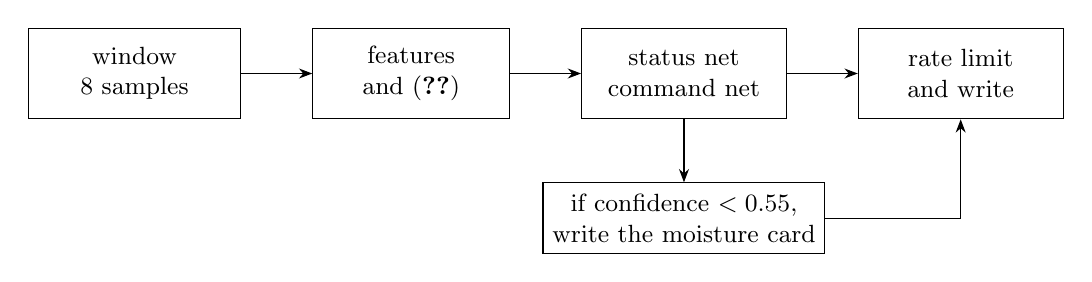
\begin{tikzpicture}[>=Stealth,node distance=7mm,font=\small]
  \node[draw,align=center,minimum width=2.7cm,minimum height=1.15cm] (w) {window\\8 samples};
  \node[draw,align=center,right=9mm of w,minimum width=2.5cm,minimum height=1.15cm] (f) {features\\and \eqref{eq:std}};
  \node[draw,align=center,right=9mm of f,minimum width=2.6cm,minimum height=1.15cm] (n) {status net\\command net};
  \node[draw,align=center,right=9mm of n,minimum width=2.6cm,minimum height=1.15cm] (a) {rate limit\\and write};
  \draw[->] (w) -- (f);
  \draw[->] (f) -- (n);
  \draw[->] (n) -- (a);
  \node[draw,align=center,below=8mm of n,minimum width=3.4cm,minimum height=0.9cm] (g) {if confidence \(<0.55\),\\write the moisture card};
  \draw[->] (n) -- (g);
  \draw[->] (g.east) -| (a.south);
\end{tikzpicture}
\caption{The onboard path. The teacher that produced \(\mathbf{u}^\star\) is not in this figure. The confidence gate selects between the command network and the moisture card of \eqref{eq:card}.}
\label{fig:exec}
\end{figure}

The tasks and the periods are fixed in advance. Nothing in the executive is a general-purpose scheduler, because a late feature build must not be free to delay the write by an unbounded amount \cite{astrom2008}.

\begin{table}[ht]
\centering
\caption{Cyclic tasks. Periods are the rates the numerical program steps at. Budgets are operation counts, not measured times on an embedded board.}
\label{tab:tasks}
\small
\begin{tabular}{@{}lllp{4.3cm}@{}}
\toprule
Task & Period & Work & Writes \\
\midrule
Acquire & \(50\,\mathrm{ms}\) & one sample into an 8-deep window & window, fault bits \\
Features & \(200\,\mathrm{ms}\) & means, deviations, contrast, \eqref{eq:std} & \(\tilde{\mathbf{x}}\) \\
Status & \(200\,\mathrm{ms}\) & \(2885\)-parameter softmax net & label, confidence \\
Command & \(200\,\mathrm{ms}\) & \(7908\)-parameter net, \(7744\) multiply-adds & \(\hat{\mathbf{u}}\), or the card \\
Write & \(200\,\mathrm{ms}\) & clip the step to \(0.08\) on each component & the plant command \\
\bottomrule
\end{tabular}
\end{table}

A desktop timing of the command net, batched in the same NumPy implementation that trained it, is well under a millisecond per window. That figure is not a board measurement and is not used as one. The operation count is the fact the period has to dominate. Seven thousand multiply-adds are two orders of magnitude inside a \(200\,\mathrm{ms}\) step on any processor that would be chosen to host this net. The reason for the cap is the rate limit and the window, not the arithmetic. The teacher, by contrast, is a grid plus an iterative solve and is not a candidate for the step. That difference is why Problem~2 is an imitation problem.

\subsection{Channels the executive consumes}

Table~\ref{tab:chan} is the measurement vector of requirement R1, written as channels rather than as a wiring diagram. The four axial stations are the installed set \(\{1,4,5,8\}\). The other channels are the scalars of Section~\ref{sec:place}. Sampling faster than the feature task is only so the window has eight distinct values; the executive never acts at the sample rate.

\begin{table}[ht]
\centering
\caption{Channels read by the executive. ``Used'' is the rate at which a new value enters the decision.}
\label{tab:chan}
\begin{tabular}{@{}llc@{}}
\toprule
Channel & Role & Used at \\
\midrule
Loads at stations \(1,4,5,8\) & shape, level, peak & \(20\,\mathrm{Hz}\) window \\
Shaft torque & level, redundant with the loads & \(20\,\mathrm{Hz}\) \\
Housing vibration & intensity check & \(20\,\mathrm{Hz}\) \\
Sieve-loss proxy & cleaner term & \(20\,\mathrm{Hz}\) \\
Return flow & accompanies sieve loss & \(20\,\mathrm{Hz}\) \\
Shaft power & accompanies specific energy & \(20\,\mathrm{Hz}\) \\
Moisture & disturbance and card input & \(1\,\mathrm{Hz}\) \\
Offered feed & disturbance & \(20\,\mathrm{Hz}\) \\
\bottomrule
\end{tabular}
\end{table}

The command write is four normalized setpoints. Intensity, residence, cleaning, and feed admission remain the interface of Chapter~\ref{ch:back}. The executive does not convert them to a rotor speed or a sieve angle. That conversion is a property of a particular machine and is outside the claim. The rate limit of \(0.08\) per component per \(200\,\mathrm{ms}\) is the claim: a step that the numerical transient is required to obey, so a jump in the network output cannot appear as a jump in the plant.

\subsection{Faults, and the direction of the fallback}

A missing axial station is dropped from the contrast and from the coefficient of variation, and the command is held for that step. If two or more of the four installed stations are missing, the write is the moisture card until the channels return. A missing moisture reading holds the last moisture and raises a fault bit. It does not invent a dry crop, because the card would then move the wrong way. A status confidence below \(0.55\) selects the card for that step. On the test windows this gate fires on \(2.5\%\) of rows. The seasonal runs and the slug in Section~\ref{sec:eval} do not inject missing channels, and they do not take the gate's credit. They are the networks with a full window. The gate is specified so that a low-confidence window has a defined output; it is not secretly responsible for the loss reduction in the tables.

The card is the fallback in every one of these cases, rather than the fixed setting or a zero command. The card is a function of moisture, it is always defined, and Chapter~\ref{ch:method} already measured it. Falling back to a command that has not been measured would make the fault logic a third controller.

\subsection{The season the program is scored on}

Eight steady points and one transient are the evaluation. The points, the feeds, the moistures, and the weights are in Table~\ref{tab:points}. The weights sum to one. They describe a wheat-heavy mix with a real rice and soybean share. They are not a yield census. The transient is wheat at moisture \(0.17\), with offered feed
\begin{equation}
q(t) = 5.0 + 3.2\exp\!\big(-{\textstyle\frac12}((t-12)/2.2)^2\big)
\label{eq:slug}
\end{equation}
from \(t=0\) to \(t=26\,\mathrm{s}\), sampled every \(0.2\,\mathrm{s}\). The crest is about \(8.2\,\mathrm{kg\,s^{-1}}\). The network starts on the card, fills the window, and is then rate-limited. The fixed command and the card are run on the same \(q(t)\) with no rate limit, because they do not move.

\begin{table}[ht]
\centering
\caption{Seasonal points. Feed is offered biomass. Weights sum to one.}
\label{tab:points}
\begin{tabular}{@{}lcccc@{}}
\toprule
Point & Crop & Feed (\(\mathrm{kg\,s^{-1}}\)) & Moisture & Weight \\
\midrule
Wheat, nominal & wheat & 6.0 & 0.145 & 0.22 \\
Wheat, wet & wheat & 6.0 & 0.220 & 0.14 \\
Wheat, dry and heavy & wheat & 8.0 & 0.120 & 0.12 \\
Wheat, light & wheat & 3.5 & 0.160 & 0.10 \\
Rice, nominal & rice & 5.0 & 0.180 & 0.14 \\
Rice, wet & rice & 6.4 & 0.250 & 0.12 \\
Soybean, nominal & soybean & 4.5 & 0.130 & 0.10 \\
Soybean, wet & soybean & 4.2 & 0.180 & 0.06 \\
\bottomrule
\end{tabular}
\end{table}

\section{Performance Evaluation}
\label{sec:eval}

\subsection{Seasonal means}

Table~\ref{tab:season} is the weighted mean of the eight points. Five policies are columns because five different questions would otherwise be collapsed. Fixed is the setting an operator leaves alone. The card is the moisture schedule \eqref{eq:card}. Linear is the least-squares imitator. Network is the deep imitator in the executive, without the rate limit, because these points are steady. Oracle is the teacher with the true disturbance. The network column is the one Problem~2 asked for. The oracle column is the ceiling of the imitation, not a field target.

\begin{table}[ht]
\centering
\caption{Weighted seasonal means. Loss terms and impurity and breakage are percent. Energy is \(\mathrm{kWh\,t^{-1}}\). Power is kilowatts.}
\label{tab:season}
\begin{tabular}{@{}lrrrrr@{}}
\toprule
Quantity & Fixed & Card & Linear & Network & Oracle \\
\midrule
Grain loss (\%) & 2.85 & 2.50 & 1.88 & 1.80 & 1.78 \\
Unthreshed (\%) & 0.93 & 0.76 & 0.53 & 0.49 & 0.47 \\
Free grain (\%) & 1.06 & 0.93 & 0.77 & 0.75 & 0.74 \\
Sieve loss (\%) & 0.86 & 0.82 & 0.58 & 0.57 & 0.57 \\
Recovery (\%) & 97.15 & 97.50 & 98.07 & 98.13 & 98.22 \\
Impurity (\%) & 1.17 & 1.20 & 1.50 & 1.50 & 1.50 \\
Breakage (\%) & 1.04 & 1.17 & 1.43 & 1.49 & 1.51 \\
Specific energy & 1.41 & 1.47 & 1.60 & 1.63 & 1.64 \\
Load CV & 0.140 & 0.127 & 0.109 & 0.104 & 0.105 \\
Peak load (N) & 969 & 952 & 930 & 928 & 929 \\
Stability \(S\) & 0.686 & 0.696 & 0.702 & 0.701 & 0.700 \\
Shaft power (kW) & 13.1 & 13.6 & 14.9 & 15.2 & 15.2 \\
\bottomrule
\end{tabular}
\end{table}

Grain loss falls from \(2.85\%\) at the fixed setting to \(2.50\%\) on the card and to \(1.80\%\) with the network. The teacher sits at \(1.78\%\). The network is within \(0.03\) points of the teacher and \(0.08\) points under the linear imitator. Recovery moves with loss because the feed trim stays open: the seasonal recovery and the complement of seasonal loss differ by less than a tenth of a point in every learned column. The network is not buying the table by refusing crop.

The prices move in the direction \(J\) told them to move. Specific energy rises from \(1.41\) to \(1.63\,\mathrm{kWh\,t^{-1}}\), shaft power from \(13.1\) to \(15.2\,\mathrm{kW}\), impurity from \(1.17\%\) to \(1.50\%\), and breakage from \(1.04\%\) to \(1.49\%\). The teacher's own column is \(1.64\), \(1.50\%\), and \(1.51\%\). The network is copying the teacher's purchase, not inventing a cheaper one. Stability rises from \(0.686\) to \(0.701\), which is the floor. A mean of \(0.701\) can hide a point that is far under the floor and another that is far over it. The point table is where that question is answered.

The card deserves a plain reading. It beats the fixed setting on the mean, by \(0.35\) points of loss, and it spends a little energy and a little breakage to do it. It is a real policy. The network's further \(0.70\) points are the part of the problem the card cannot see: feed, packing, and the load shape.

\subsection{Point by point}

Table~\ref{tab:pointsfull} gives loss, stability, and specific energy at each point for the fixed setting, the card, the network, and the teacher. The linear map is omitted here because its seasonal mean is already in Table~\ref{tab:season} and the point-level story is about whether the network tracked the teacher where the card fails.

\begin{table}[ht]
\centering
\caption{Loss (\%), stability \(S\), and specific energy at each seasonal point.}
\label{tab:pointsfull}
\small
\setlength{\tabcolsep}{4pt}
\begin{tabular}{@{}lrrrrrrrrrrrr@{}}
\toprule
& \multicolumn{3}{c}{Fixed} & \multicolumn{3}{c}{Card} & \multicolumn{3}{c}{Network} & \multicolumn{3}{c}{Oracle} \\
\cmidrule(lr){2-4}\cmidrule(lr){5-7}\cmidrule(lr){8-10}\cmidrule(lr){11-13}
Point & \(L\) & \(S\) & \(e\) & \(L\) & \(S\) & \(e\) & \(L\) & \(S\) & \(e\) & \(L\) & \(S\) & \(e\) \\
\midrule
Wheat nom. & 2.46 & 0.71 & 1.33 & 2.44 & 0.72 & 1.33 & 1.57 & 0.70 & 1.55 & 1.54 & 0.70 & 1.56 \\
Wheat wet & 3.40 & 0.65 & 1.54 & 2.61 & 0.67 & 1.70 & 2.07 & 0.70 & 1.80 & 2.01 & 0.70 & 1.82 \\
Wheat heavy & 2.65 & 0.64 & 1.29 & 2.85 & 0.64 & 1.25 & 1.57 & 0.72 & 1.54 & 1.96 & 0.70 & 1.39 \\
Wheat light & 1.93 & 0.76 & 1.32 & 1.83 & 0.77 & 1.35 & 1.50 & 0.70 & 1.46 & 1.52 & 0.70 & 1.45 \\
Rice nom. & 3.00 & 0.72 & 1.46 & 2.65 & 0.73 & 1.54 & 1.99 & 0.69 & 1.69 & 1.86 & 0.70 & 1.73 \\
Rice wet & 4.99 & 0.54 & 1.70 & 3.37 & 0.56 & 1.94 & 2.65 & 0.70 & 2.07 & 2.27 & 0.70 & 2.19 \\
Soy nom. & 1.83 & 0.76 & 1.23 & 1.90 & 0.76 & 1.21 & 1.41 & 0.70 & 1.34 & 1.42 & 0.70 & 1.33 \\
Soy wet & 2.06 & 0.76 & 1.36 & 1.84 & 0.76 & 1.43 & 1.56 & 0.71 & 1.49 & 1.54 & 0.70 & 1.51 \\
\bottomrule
\end{tabular}
\end{table}

Three rows carry the argument. The others are the same pattern at a smaller scale.

On nominal wheat the card and the fixed setting are the same policy for practical purposes, loss \(2.46\%\) and \(2.44\%\), because the card was written to pass near the fixed setting at moderate moisture. The network lowers loss to \(1.57\%\), against the teacher's \(1.54\%\), and raises energy from \(1.33\) to \(1.55\,\mathrm{kWh\,t^{-1}}\). Stability was already at the floor and stays there. The command the network writes is \((0.69,\ 0.55,\ 0.65,\ 1.00)\), against the teacher's \((0.70,\ 0.55,\ 0.65,\ 1)\). Intensity and cleaning rise. Residence rises a little. The feed trim does not move.

On dry, heavy wheat the card is worse than the fixed setting: loss \(2.85\%\) against \(2.65\%\), energy slightly down. Low moisture tells the card to ease off, and the heavy feed is invisible to it. The teacher goes the other way on residence, to \(0.59\), and holds intensity at \(0.50\), with loss \(1.96\%\) and energy \(1.39\). The network overshoots that instruction. It writes \((0.59,\ 0.71,\ 0.68,\ 1)\), loss \(1.57\%\), energy \(1.54\), breakage \(1.63\%\) against the teacher's breakage of \(1.27\%\). Loss looks better than the teacher and the objective does not, because breakage and energy were the terms the teacher refused to spend. This is the row where imitation error is visible as a purchase, not as a random residual. It is also the row that shows why a loss-only table would have ranked the network above the teacher and been wrong about \(J\).

On wet rice the fixed setting loses \(4.99\%\), sits at stability \(0.54\), and peaks at \(1441\,\mathrm{N}\), which is over the blockage line of \(1411\,\mathrm{N}\). The card cuts loss to \(3.37\%\) and leaves stability at \(0.56\). The teacher raises residence to \(0.85\) and intensity to \(0.63\), cuts loss to \(2.27\%\), brings the peak down to \(1163\,\mathrm{N}\), and pays with breakage \(3.36\%\) and energy \(2.19\,\mathrm{kWh\,t^{-1}}\). The network writes \((0.56,\ 0.80,\ 0.66,\ 1)\). Loss is \(2.65\%\), stability \(0.70\), peak load \(1182\,\mathrm{N}\), breakage \(2.96\%\), energy \(2.07\). It reaches the floor and it does not reach the teacher's loss. The gap of \(0.38\) points is the largest point-level gap in the table. The load coefficient of variation on this row falls from \(0.157\) at the fixed setting to \(0.047\) under the network. That is the shape term doing the work the card cannot do, and it is why the middle-and-end placement is in the feature vector even though two stations already classify the label.

On light wheat the fixed setting is already above the floor, at \(0.76\). The teacher spends the margin down to \(0.70\), lowers residence to \(0.37\), and cuts loss from \(1.93\%\) to \(1.52\%\). The network does the same thing: residence \(0.38\), loss \(1.50\%\), stability \(0.70\). Extra residence is not a universal command. The objective's hinge is the reason. Above \(0.70\), further calmness is unpaid, and a light crop should not be held longer for a calmness the cost does not buy.

Feed admission stays at \(1\), or within \(0.01\) of \(1\), on every seasonal point and for both the network and the teacher. The trim is in the command vector because the plant allows it and because a policy that used it would be visible in the recovery column. Neither the teacher nor the imitator needs it on this mix. The blockage hinge is met by residence and intensity instead. A heavier point than wet rice could move the trim. No such point is in the weighted mean, and none is added after the fact.

\subsection{The feed transient}

The slug of \eqref{eq:slug} asks whether a rate-limited network, which at \(t=0\) is still equal to the card, gives the steady-state gain back when the feed rises for a few seconds. Figure~\ref{fig:slug} is the peak station load. Table~\ref{tab:slug} is the same run at the crest and at the two shoulders.

\begin{figure}[ht]
\centering
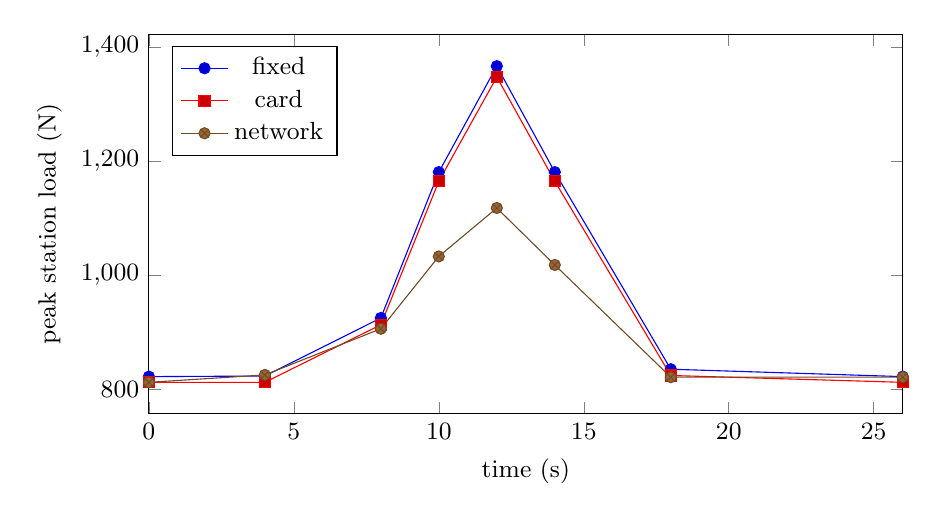
\begin{tikzpicture}
\begin{axis}[
  width=0.92\textwidth,
  height=6.4cm,
  xlabel={time (s)},
  ylabel={peak station load (N)},
  xmin=0, xmax=26,
  legend style={font=\small,at={(0.03,0.97)},anchor=north west},
]
\addplot coordinates {
(0,822) (4,823) (8,925) (10,1181) (12,1367) (14,1181) (18,835) (26,822)
};
\addplot coordinates {
(0,812) (4,812) (8,913) (10,1165) (12,1348) (14,1165) (18,824) (26,812)
};
\addplot coordinates {
(0,812) (4,825) (8,906) (10,1033) (12,1118) (14,1018) (18,821) (26,821)
};
\legend{fixed,card,network}
\end{axis}
\end{tikzpicture}
\caption{Peak station load through the wheat feed transient at moisture \(0.17\). The offer peaks near \(8.2\,\mathrm{kg\,s^{-1}}\) at \(t=12\,\mathrm{s}\). The network is rate-limited and starts on the card.}
\label{fig:slug}
\end{figure}

\begin{table}[ht]
\centering
\caption{Wheat transient at moisture \(0.17\). Loss is percent. Peak load is newtons.}
\label{tab:slug}
\begin{tabular}{@{}rrrrrrrr@{}}
\toprule
& & \multicolumn{2}{c}{Fixed} & \multicolumn{2}{c}{Card} & \multicolumn{2}{c}{Network} \\
\cmidrule(lr){3-4}\cmidrule(lr){5-6}\cmidrule(lr){7-8}
\(t\) (s) & Feed & Loss & Peak & Loss & Peak & Loss & Peak \\
\midrule
0 & 5.00 & 2.43 & 822 & 2.22 & 812 & 2.22 & 812 \\
4 & 5.00 & 2.43 & 823 & 2.23 & 812 & 1.44 & 825 \\
8 & 5.61 & 2.59 & 925 & 2.37 & 913 & 1.55 & 906 \\
12 & 8.20 & 3.19 & 1367 & 2.92 & 1348 & 1.81 & 1118 \\
18 & 5.08 & 2.45 & 835 & 2.24 & 824 & 1.33 & 821 \\
26 & 5.00 & 2.43 & 822 & 2.22 & 812 & 1.49 & 821 \\
\bottomrule
\end{tabular}
\end{table}

At \(t=0\) the network has not moved, and its loss equals the card. By \(t=4\,\mathrm{s}\), still before the crest, loss is \(1.44\%\) and the command has walked to about \((0.74,\ 0.58,\ 0.63,\ 1)\). At the crest the fixed peak is \(1367\,\mathrm{N}\) and the network peak is \(1118\,\mathrm{N}\). Fixed loss is \(3.19\%\) and network loss is \(1.81\%\). The load coefficient of variation at the crest is \(0.141\) for the fixed command and \(0.026\) for the network: residence has risen to \(0.84\), which is the same direction the teacher used on wet, heavy steady points. Minimum stability over the twenty-six seconds is \(0.586\) for the fixed command, \(0.597\) for the card, and \(0.701\) for the network. Mean loss over the transient is \(2.59\%\), \(2.38\%\), and \(1.48\%\).

The rate limit is what makes the four-second delay in Table~\ref{tab:slug} a real delay rather than a skipped sample. A command that jumped from the card to the crest command in one step would have produced the same crest numbers and would have violated the write rule in Table~\ref{tab:tasks}. The plotted run does not do that. From \(t=4\) to \(t=12\) residence moves from \(0.58\) to \(0.84\) while the feed is rising, which is several capped steps, not one.

\subsection{What the evaluation does and does not establish}

The evaluation establishes four comparisons on this plant, at the published weights of \eqref{eq:J}, with seed \(7\).

The status network on the installed placement is more accurate than a linear softmax on the features the placement makes, and the margin is in the spatial and the rare classes. That result belongs to Chapter~\ref{ch:method} and is not re-litigated by the loss tables. A season can look good while the labeler is weak, because the command net never reads the label.

The command network reproduces the teacher's seasonal loss to \(0.03\) points and the teacher's energy, impurity, and breakage to a few hundredths. A linear imitator of the same teacher recovers most of the same gain and leaves \(0.08\) points more loss on the seasonal mean. Depth is a small advantage on the command once the features exist. It is not zero on this mix, and it is not the reason the card loses.

The moisture card is a lawful baseline. It helps on wet wheat and on wet rice, and it hurts on dry, heavy wheat. Any summary that reports only the seasonal mean of the card will call it a modest improvement and will miss the row it gets backwards.

The stability floor is met as a seasonal mean and as a minimum along the tested transient. It is not met as a hard constraint on every random test window: Chapter~\ref{ch:method} recorded that \(30\%\) of those windows still fall just under \(0.70\) after imitation, against \(0.4\%\) for the teacher. The tenth percentile on that mixture is \(0.693\). The executive does not project \(\hat{\mathbf{u}}\) back onto \(\{S\ge 0.70\}\). Doing so would require the plant inside the step, which is the teacher again. The gap is the price of a pure function evaluation, and it should be read as a gap.

The evaluation does not establish a field loss of \(1.80\%\). The plant was built so that a fixed command would sit in a published band of axial loss and specific energy, and so that feed and moisture would interact. A different breakage weight would move the dry-heavy overshoot and the wet-rice purchase. The same comparison, at these weights, is what the tables are for: a fixed setting and a moisture card, against a network that imitates a cost in which those purchases are explicit, with the teacher present in the last column so the imitation can be seen to succeed and, on two rows, to miss.

\begin{thebibliography}{99}

\bibitem{goodfellow2016}
I.~Goodfellow, Y.~Bengio, and A.~Courville,
\emph{Deep Learning}.
Cambridge, MA, USA: MIT Press, 2016.

\bibitem{lecun2015}
Y.~LeCun, Y.~Bengio, and G.~Hinton,
``Deep learning,''
\emph{Nature}, vol.~521, pp.~436--444, 2015.

\bibitem{rumelhart1986}
D.~E. Rumelhart, G.~E. Hinton, and R.~J. Williams,
``Learning representations by back-propagating errors,''
\emph{Nature}, vol.~323, pp.~533--536, 1986.

\bibitem{cybenko1989}
G.~Cybenko,
``Approximation by superpositions of a sigmoidal function,''
\emph{Mathematics of Control, Signals and Systems}, vol.~2, pp.~303--314, 1989.

\bibitem{hornik1991}
K.~Hornik,
``Approximation capabilities of multilayer feedforward networks,''
\emph{Neural Networks}, vol.~4, no.~2, pp.~251--257, 1991.

\bibitem{he2015}
K.~He, X.~Zhang, S.~Ren, and J.~Sun,
``Delving deep into rectifiers: Surpassing human-level performance on ImageNet classification,''
in \emph{Proc. IEEE Int. Conf. Computer Vision}, 2015, pp.~1026--1034.

\bibitem{kingma2015}
D.~P. Kingma and J.~Ba,
``Adam: A method for stochastic optimization,''
in \emph{Proc. Int. Conf. Learning Representations}, 2015.

\bibitem{bishop2006}
C.~M. Bishop,
\emph{Pattern Recognition and Machine Learning}.
New York, NY, USA: Springer, 2006.

\bibitem{hastie2009}
T.~Hastie, R.~Tibshirani, and J.~Friedman,
\emph{The Elements of Statistical Learning}, 2nd~ed.
New York, NY, USA: Springer, 2009.

\bibitem{atkinson2007}
A.~C. Atkinson, A.~N. Donev, and R.~D. Tobias,
\emph{Optimum Experimental Designs, with SAS}.
Oxford, U.K.: Oxford University Press, 2007.

\bibitem{nocedal2006}
J.~Nocedal and S.~J. Wright,
\emph{Numerical Optimization}, 2nd~ed.
New York, NY, USA: Springer, 2006.

\bibitem{boyd2004}
S.~Boyd and L.~Vandenberghe,
\emph{Convex Optimization}.
Cambridge, U.K.: Cambridge University Press, 2004.

\bibitem{ross2011}
S.~Ross, G.~J. Gordon, and J.~A. Bagnell,
``A reduction of imitation learning and structured prediction to no-regret online learning,''
in \emph{Proc. Int. Conf. Artificial Intelligence and Statistics}, 2011, pp.~627--635.

\bibitem{astrom2008}
K.~J. {\AA}str\"om and R.~M. Murray,
\emph{Feedback Systems: An Introduction for Scientists and Engineers}.
Princeton, NJ, USA: Princeton University Press, 2008.

\bibitem{rawlings2017}
J.~B. Rawlings, D.~Q. Mayne, and M.~M. Diehl,
\emph{Model Predictive Control: Theory, Computation, and Design}, 2nd~ed.
Madison, WI, USA: Nob Hill, 2017.

\bibitem{kamilaris2018}
A.~Kamilaris and F.~X. Prenafeta-Bold\'u,
``Deep learning in agriculture: A survey,''
\emph{Computers and Electronics in Agriculture}, vol.~147, pp.~70--90, 2018.

\bibitem{liakos2018}
K.~G. Liakos, P.~Busato, D.~Moshou, S.~Pearson, and D.~Bochtis,
``Machine learning in agriculture: A review,''
\emph{Sensors}, vol.~18, no.~8, art.~2674, 2018.

\bibitem{patricio2018}
D.~I. Patr\'icio and R.~Rieder,
``Computer vision and artificial intelligence in precision agriculture for grain crops: A systematic review,''
\emph{Computers and Electronics in Agriculture}, vol.~153, pp.~69--81, 2018.

\bibitem{chen2025}
Z.~Chen, Z.~Qian, C.~Jin, and T.~Yang,
``Research progress on control algorithms for grain combine harvesters,''
\emph{Applied Sciences}, vol.~15, no.~16, art.~9176, 2025.

\bibitem{craessaerts2010a}
G.~Craessaerts, J.~De~Baerdemaeker, B.~Missotten, and W.~Saeys,
``Fuzzy control of the cleaning process on a combine harvester,''
\emph{Biosystems Engineering}, vol.~106, no.~2, pp.~103--111, 2010.

\bibitem{coen2008b}
T.~Coen, W.~Saeys, B.~Missotten, and J.~De~Baerdemaeker,
``Cruise control on a combine harvester using model-based predictive control,''
\emph{Biosystems Engineering}, vol.~99, no.~1, pp.~47--55, 2008.

\bibitem{liang2016}
Z.~Liang, Y.~Li, L.~Xu, and Z.~Zhao,
``Sensor for monitoring rice grain sieve losses in combine harvesters,''
\emph{Biosystems Engineering}, vol.~147, pp.~51--66, 2016.

\bibitem{zhao2011}
Z.~Zhao, Y.~Li, J.~Chen, and J.~Xu,
``Grain separation loss monitoring system in combine harvester,''
\emph{Computers and Electronics in Agriculture}, vol.~76, no.~2, pp.~183--188, 2011.

\bibitem{miu2008a}
P.~I. Miu and H.-D. Kutzbach,
``Modeling and simulation of grain threshing and separation in threshing units---Part I,''
\emph{Computers and Electronics in Agriculture}, vol.~60, no.~1, pp.~96--104, 2008.

\bibitem{harrison1991}
H.~P. Harrison,
``Rotor power and losses of an axial-flow combine,''
\emph{Transactions of the ASAE}, vol.~34, no.~1, pp.~60--64, 1991.

\bibitem{srivastava2006}
A.~K. Srivastava, C.~E. Goering, R.~P. Rohrbach, and D.~R. Buckmaster,
\emph{Engineering Principles of Agricultural Machines}, 2nd~ed.
St.~Joseph, MI, USA: ASABE, 2006.

\bibitem{kepner1978}
R.~A. Kepner, R.~Bainer, and E.~L. Barger,
\emph{Principles of Farm Machinery}, 3rd~ed.
Westport, CT, USA: AVI, 1978.

\bibitem{fu2018}
J.~Fu, Z.~Chen, L.~Han, and L.~Ren,
``Review of grain threshing theory and technology,''
\emph{International Journal of Agricultural and Biological Engineering}, vol.~11, no.~3, pp.~12--20, 2018.

\end{thebibliography}


\end{document}
